The general equation of a second degree can be expressed as: 
\begin{align}
   \vec{x}^T\vec{V}\vec{x}+2\vec{u}^T\vec{x}+f=0 \label{eq:solutions/41/8/eq:conic}
\end{align}
Comparing \eqref{eq:solutions/41/8/eq:given} and \eqref{eq:solutions/41/8/eq:conic}
\begin{align}
\vec{V}=\vec{V}^T =\myvec{16 & -12 \\ -12 & 9 }, \quad\vec{u}=\myvec{16 \\ 43},\quad f=-39 \label{eq:solutions/41/8/eq:parametrics}
\end{align}
{Eigen Values:}
The characteristic equation of $\vec{V}$ is given as
\begin{align}
\mydet{\lambda \vec{I}-\vec{V}} = 0
\end{align}
\begin{align}
\implies \mydet{\lambda-16 & 12 \\ 12 & \lambda-9} =0
\end{align}
\begin{align}
\implies \lambda^2-25\lambda=0 \label{eq:solutions/41/8/eq:chartistic}
\end{align}
The eigenvalues are the roots of the equation \eqref{eq:solutions/41/8/eq:chartistic}, which are as follows:
\begin{align}
 \lambda_1=0, \quad  \lambda_2=25 \label{eq:solutions/41/8/eq:eigenval}
\end{align}
{Eigen Vectors:}
The eigen vector $\vec{p}$ is defined as
\begin{align}
\vec{V}\vec{p}=\lambda\vec{p}     
\end{align}
\begin{align}
\implies (\lambda \vec{I} - \vec{V} ) \vec{p} = 0
\end{align}
For $\lambda_1 = 0 $
\begin{align}
(\lambda_1 \vec{I}-\vec{V} ) = \myvec{-16 & 12 \\ 12 & -9 }\xleftrightarrow[R_2\leftarrow R_2+3R_1]{R_1\leftarrow \frac{1}{4}R_1}\myvec{-4 & 3\\0 & 0}
\end{align}
\begin{align}
\implies \vec{p_1} = \frac{1}{5} \myvec{3 \\ 4} \label{eq:solutions/41/8/eq:p1val}
\end{align}
For $\lambda_2 = 25$
\begin{align}
(\lambda_2 \vec{I}-\vec{V} ) = \myvec{9 & 12 \\ 12 & 1}\xleftrightarrow[R_2\leftarrow R_2-4R_1]{R_1\leftarrow \frac{1}{3}R_1}\myvec{3 & 4\\0 & 0}
\end{align}
\begin{align}
\implies \vec{p_2} = \frac{1}{5} \myvec{-4\\ 3} \label{eq:solutions/41/8/eq:p2val}
\end{align}
{Eigen Value Decomposition:}
Using EVD, we can write 
\begin{align}
 \vec{D} = \vec{P} \vec{V} \vec{P}^T
\end{align}
From \eqref{eq:solutions/41/8/eq:p1val} and \eqref{eq:solutions/41/8/eq:p2val}
\begin{align}
 \vec{P} = \frac{1}{5} \myvec{3 & -4 \\ 4 & 3}
\end{align}
From \eqref{eq:solutions/41/8/eq:eigenval}
\begin{align}
 \vec{D} = \myvec{\lambda_1 & 0 \\ 0 & \lambda_2} = \myvec{0 & 0 \\ 0 & 25}
\end{align}
{Parabola}
\begin{align}
\text{Focal Length} = \abs{\frac{2\eta}{\lambda_2}} \label{eq:solutions/41/8/eq:focallen}\\
\intertext{From \eqref{eq:solutions/41/8/eq:p1val} and \eqref{eq:solutions/41/8/eq:parametrics}}
\eta = \vec{p}_1^T\vec{u} = 44 \label{eq:solutions/41/8/eq:etaval}\\
\intertext{Substituting values of \eqref{eq:solutions/41/8/eq:etaval} and \eqref{eq:solutions/41/8/eq:eigenval} in \eqref{eq:solutions/41/8/eq:focallen}, we get}
\text{Focal Length} = \abs{\frac{88}{25}}=3.52
\end{align}
The standard equation of parabola is given by:
\begin{align}
 \vec{y}^T\vec{D}\vec{y} = -2\eta \myvec{1 & 0}\vec{y} \label{eq:solutions/41/8/eq:parabola}
\end{align}
And the vertex $\vec{c}$ is:
\begin{align}
 \myvec{\vec{u}^T+\eta \vec{p_1}^T \\ \vec{V}}\vec{c} = \myvec{-f \\ \eta \vec{p_1}-\vec{u}}
\end{align}
From \eqref{eq:solutions/41/8/eq:parametrics} \eqref{eq:solutions/41/8/eq:etaval} and \eqref{eq:solutions/41/8/eq:p1val},
\begin{align}
\myvec{\frac{212}{5} & \frac{391}{5} \\ 16 & -12 \\ -12 & 9}\vec{c}=\myvec{39 \\ \frac{52}{5}\\ \frac{-39}{5}}
\end{align}
To find $\vec{c}$, perform row reduction on the augmented matrix as follows:
\begin{align}
    \myvec{\frac{212}{5} & \frac{391}{5} & 39\\16 & -12 & \frac{52}{5}\\-12 & 9 & \frac{-39}{5}}\xleftrightarrow[R_1\leftarrow \frac{5}{212}R_1]{R_3\leftarrow R_3+\frac{3}{4}R_2}\myvec{1 & \frac{391}{212} & \frac{195}{212}\\16 & -12 & \frac{52}{5}\\0&0&0}\\
    \xleftrightarrow{R_2\leftarrow R_2-16R_1}\myvec{ 1 & \frac{391}{212} & \frac{195}{212}\\0 & \frac{-2200}{53} & \frac{-1144}{265} \\0&0&0}\\\xleftrightarrow{R_2\leftarrow \frac{-53}{2200}R_2}\myvec{1 & \frac{391}{212} & \frac{195}{212} \\0 & 1 & \frac{13}{125}\\0&0&0}\\\xleftrightarrow{R_1\leftarrow R_1-\frac{391}{212}R_2}\myvec{1 & 0 & \frac{4823}{6625}\\0 & 1 & \frac{13}{125}\\0&0&0}
\end{align}
Hence,
\begin{align}
\vec{c}=\myvec{\frac{4823}{6625}\\ \frac{13}{125}}= \myvec{0.728 \\ 0.104}
\end{align}
\begin{figure}[h!]
	\centering
	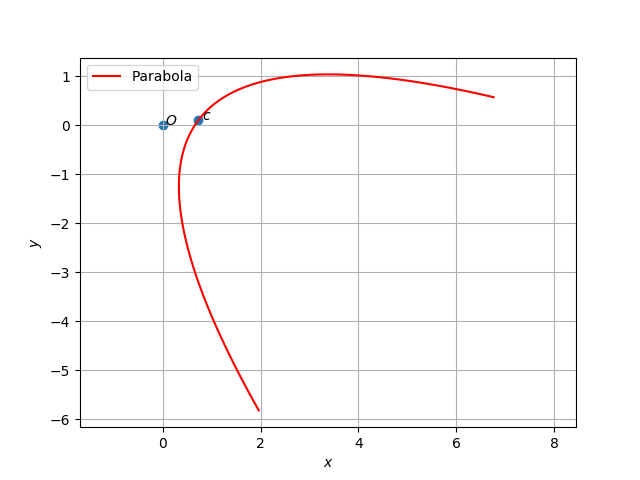
\includegraphics[width=\columnwidth]{./solutions/41/8/Codes/A5.png}
	\caption{Parabola with vertex c }
	\label{eq:solutions/41/8/myfig}
\end{figure}
